\documentclass[t]{beamer}
\usepackage[utf8]{inputenc}
\usepackage{soul}
\usepackage{tabularx}
\usepackage{booktabs}
\usepackage{tikz}
\usepackage{ulem}
\usepackage[per-mode = symbol,detect-all=true]{siunitx}
\sisetup{
    output-decimal-marker = {.},
    output-exponent-marker=\textsc{e}, 
    % round-mode=places,
    output-complex-root=j, 
    % unit-color=blue,
    % scientific-notation = engineering
}
\DeclareSIUnit[number-unit-product = \,]{\permil}{\textperthousand}
\usetheme{noergaard}
\newcommand{\hi}[1]{{\textcolor{themecolor}{\bfseries{#1}}}}

\definecolor{bb}{rgb}{0.0, 0.0, 1.0}
\definecolor{gg}{rgb}{0.0, 0.5, 0.0}
\definecolor{rr}{rgb}{1.0, 0.0, 0.0}
\definecolor{cc}{rgb}{0.0, 0.75, 0.75}
\definecolor{mm}{rgb}{0.75, 0.0, 0.75}
\definecolor{yy}{rgb}{0.75, 0.75, 0.0}
\definecolor{kk}{rgb}{0.0, 0.0, 0.0}

\newcounter{funcreqcnt}
\newcounter{specreqcnt}
\newcommand{\freq}[1]{ \refstepcounter{funcreqcnt}\label{#1} F\arabic{funcreqcnt} }
\newcommand{\sreq}[1]{ \refstepcounter{specreqcnt}\label{#1} S\arabic{specreqcnt} }
\newcommand{\freqref}[1]{F\ref{#1}}
\newcommand{\sreqref}[1]{S\ref{#1}}


\title{\hi{Tunable Antennas for Handsets Supporting MIMO}}
\author{
    \hi{Group 951/1051}\\
    Henrik A.\ Vesterager\\
    Søren B.\ Nørgaard\\
    Lasse Thomsen\\[1em]
    Wireless Communication Systems\\
    Dept.\ of Electronic Systems, Aalborg University
}
\date{June 24, 2016}


\begin{document}
{%
    \setbeamertemplate{headline}{}
    \frame{\titlepage}
}

\begin{frame}
    \frametitle{Overview}
    \ \\
    \begin{minipage}{\linewidth}
        \tableofcontents
    \end{minipage}
\end{frame}

\section{Subject for TOC}
\begin{frame}
    \frametitle{Subject -- Slide 1 Title}
    \begin{block}{Sub-subject 1}
        Text and itemizes here.
    \end{block}
    \begin{block}{Sub-subject 2}
        Text and itemizes here.
    \end{block}
\end{frame}

\begin{frame}[fragile]
    \frametitle{Subject -- Slide 2 Title}
    \begin{columns}[onlytextwidth,t]
        \column{0.49\linewidth}
        \begin{block}{Subject 1}
            Text in the left column.
        \end{block}
        \begin{block}{Subject 2}
            Remember, do not use the following environments for slides! No captions!
            \begin{itemize}
                \item \texttt{figure}
                \item \texttt{table}
            \end{itemize}
        \end{block}
        \begin{block}{Highlighting}
            Use \hl{this} tag to highlight (\verb|\hl{}|).
        \end{block}

        \column{0.49\linewidth}
        \begin{center}
            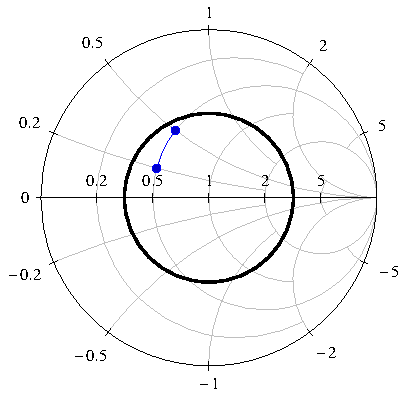
\includegraphics[scale=0.7]{img/smithchart}
        \end{center}
        Here is second column!
    \end{columns}
\end{frame}


\section{Introduction}
%Motivation
\begin{frame}
    \frametitle{Introduction -- Motivation}
    \begin{block}{Tunable Antennas}
      \begin{itemize}
      \item Even though smartphones has begun to grow in physical size, less space is allocated for the antennas.
      \item LTE standard requiresterminals to operate in a wide range of frequencies (650-2700)
      \item MIMO is a large part of LTE, which increases the number of antennas on the device 
      \item Able to make smaller antennas that can cover more bands.
      \item Approched in a very pratical manner with theory in mind. 
      \item Simple simulations and then actual prototypes.
      \end{itemize}
    \end{block}
\vspace*{-0.5cm}
  \begin{center} 
   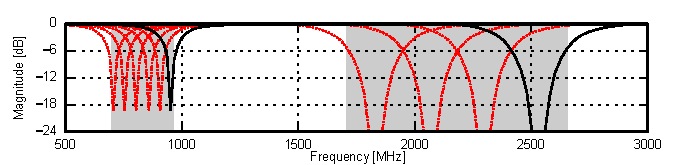
\includegraphics[width=\textwidth]{img/henrik/reconfsweep}
  \end{center}
\end{frame}
%System overview 
\begin{frame}
    \frametitle{Introduction -- A System Perspective}
  \begin{center} 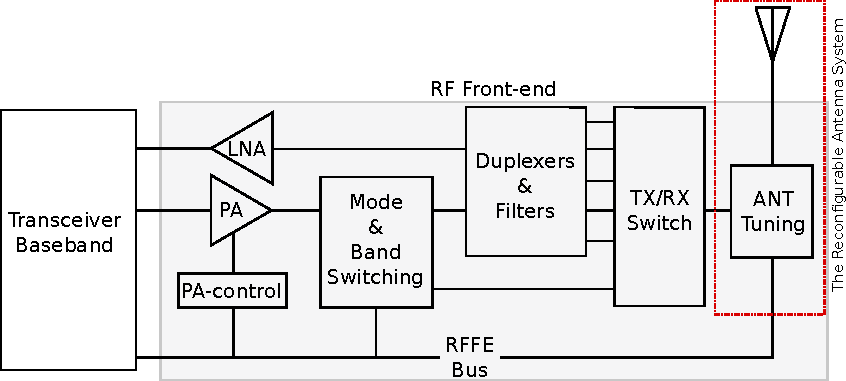
\includegraphics[scale=0.8]{img/henrik/system_diagram}
  \end{center}
\end{frame}


%Problem anal
\section{Problem Analysis}
\begin{frame}[fragile]
    \frametitle{Initial Problem Analysis}
    \vspace*{-0.5cm}
    \begin{columns}[onlytextwidth,t]
        \column{0.49\linewidth}
    \begin{block}{Topics}
          \begin{itemize}
          \item Mobile standards
          \item LTE
          \item Basic Antenna Theory
          \item Matching circuits \& Tuners
          \item Propagations Models
          \end{itemize}
    \end{block}
        \column{0.49\linewidth}
    \begin{block}{}
          \begin{itemize}
          \item User effects
          \item MIMO in Handsets
          \item Maxwell's Equations
          \item FDTD 
          \item Test Equipment and methods
          \end{itemize}
    \end{block}
    \end{columns}
    \begin{block}{Outcome of Analysis}
      \begin{itemize}
      \item Covering all the specified bands is indeed a problem
      \item Can be solved with frequency reconfigurability
      \item Correlation and isolation are important parameters for MIMO-capacity
      \item Many different types of tuners, we chose RF-mems capacitors
      \end{itemize}
    \end{block}
\end{frame}

%System overview 
\begin{frame}
    \frametitle{Requirement specification}

    \begin{block}{Functional Requirements}
    \centering
    {\tiny
\begin{tabularx}{\linewidth}{|l|X|}
    \hline
    ID & Requirement \\
    \hline
    \freq{dualband} & The antenna system must consist of two single-feed dual-band antennas covering the bands described in Requirement~\sreqref{fbands}. \\
    \freq{updownlink} & Each antenna must cover both uplink and downlink at the same time for each required LTE band.\\
    % \freq{usereffect} & Must be able to re-tune any detuning due to user effects. \\ % ???? HAHA
    \freq{matching} & Must have a simple matching network, containing a variable capacitor for tuning inside the specified bands.\\
    \freq{wispry} & Must use a WiSpry WS1040 MEMS variable capacitor chip in the matching network.\\
    \hline
\end{tabularx}

    }
    \end{block}

    \begin{block}{Specific Requirements}
    \centering
    {\tiny
\begin{tabularx}{\linewidth}{|l|l|X|}
    \hline
    ID & Specification & Requirement \\
    \hline
    \sreq{fbands} & Frequency bands\slash tunable range & \num{700}--\SI{960}{MHz}, \num{1710}--\SI{2170}{MHz}, \num{2300}--\SI{2400}{MHz}, \num{2550}--\SI{2650}{MHz} \\
    \sreq{bandwidthlow} & Minimum tunable bandwidth (\num{700}--\SI{960}{MHz}) & \SI{80}{MHz} (band 8) \\
    \sreq{bandwidthhigh} & Minimum tunable bandwidth (\num{1710}--\SI{2650}{MHz}) & \SI{720}{MHz} (band 15) \\
    \sreq{physdim} & Physical dimensions & External: $70\times140\times7$\,\si{mm\cubed}, PCB: $55\times120\times1.6$\,\si{mm\cubed} (FR-4)\\
    \sreq{copper} & Ground plane copper thickness & \SI{0.035}{mm} \\
    \sreq{retloss} & In-band return loss (impedance bandwidth) & $\text{RL} > \SI{6}{dB}$\\
    \sreq{correlation} & In-band correlation between antenna elements (correlation bandwidth) & $\rho_e < 0.5$\\
    \sreq{efficiency} & In-band total efficiency in free-space (efficiency bandwidth)  & $>\SI{50}{\%}$ \\
    \sreq{sar} & Maximum SAR & \SI{2}{W\per kg} averaged over \SI{10}{g} of tissue\\
    \sreq{tunable} & Tunable capacitor range (WS1040)& \SI{0.3}{pF} to \SI{2.9}{pF} in steps of \SI{0.2}{pF} (\SI{0.1}{pF} minimum)  \\
    \sreq{ltepower} & Reference power level  & \SI{23}{dBm} (\SI{0.2}{W})\\
    \hline
\end{tabularx}

    }
    \end{block}

    \begin{block}{Test Specification}    
      \begin{itemize}
      \item For each specific requirement is a given test specification
      \end{itemize}
    \end{block}
\end{frame}

\section{Technical Solution}
\begin{frame}
    \frametitle{Technical Solution -- Introduction}
    \begin{block}{Three different antenna designs}
      \begin{itemize}
      \item Initial designs did not have to fully comply with the requirements
      \item Some based on previous designs from published papers
      \item Simplified simulations
      \end{itemize}
    \end{block}
\vspace*{-0.5cm}
  \begin{center} 
    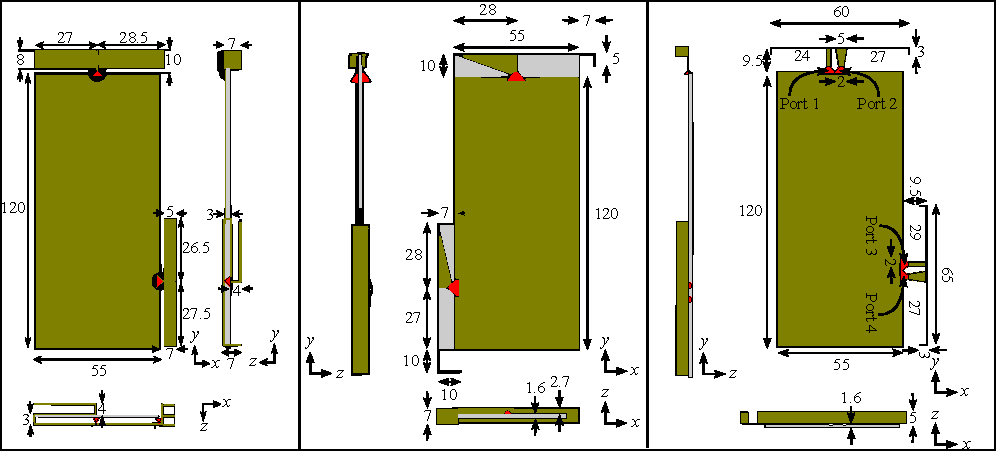
\includegraphics[width=\textwidth]{img/henrik/all_td}%

  \end{center}
\end{frame}

\section{Free-space simulations}




\begin{frame}
    \frametitle{Free-space simulations -- Monopole (S-parameters)}
    \vspace*{-0.5cm}
  \begin{minipage}[t]{0.49\linewidth}
    \vspace{0mm}

    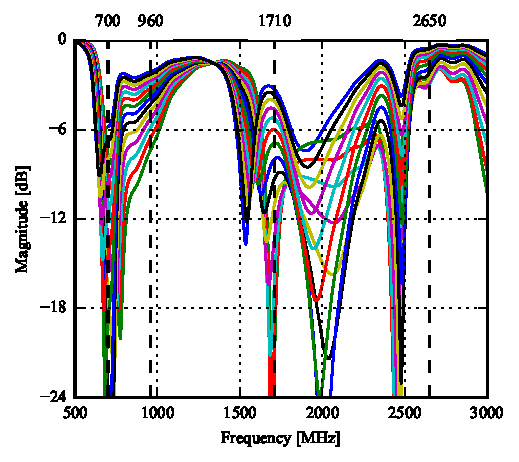
\includegraphics[width=0.78\linewidth]{img/henrik/mono/s11} \\
    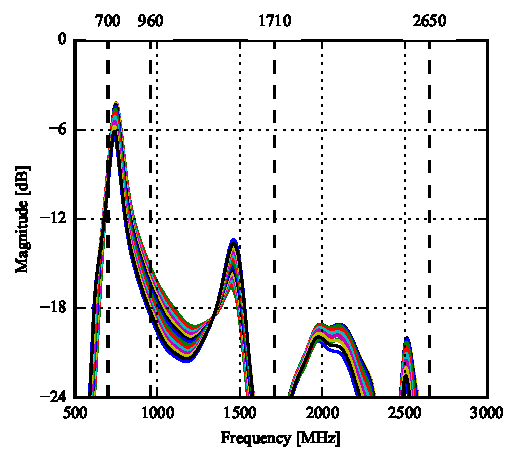
\includegraphics[width=0.78\linewidth]{img/henrik/mono/s21-s11} 

  \end{minipage}\hfill       
  \begin{minipage}[t]{0.49\linewidth}
    \vspace{0 mm}

    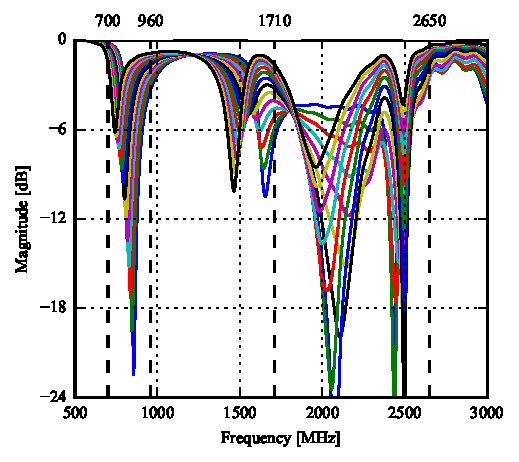
\includegraphics[width=0.78\linewidth]{img/henrik/mono/s22} \\
    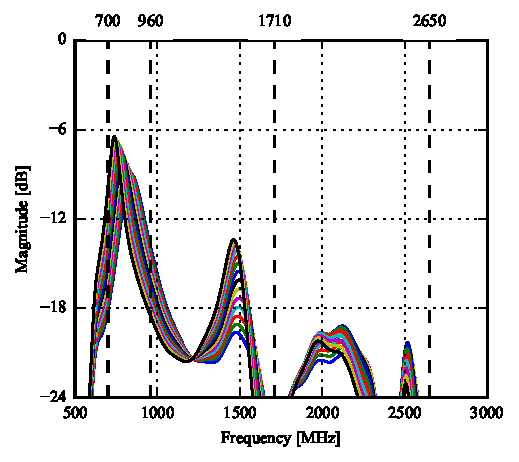
\includegraphics[width=0.78\linewidth]{img/henrik/mono/s21-s22} 

  \end{minipage}    
\end{frame}

\begin{frame}
    \frametitle{Free-space simulations -- Monopole (Efficiency and correlation)}
    \vspace*{-0.5cm}
  \begin{minipage}[t]{0.49\linewidth}
    \vspace{0mm}

    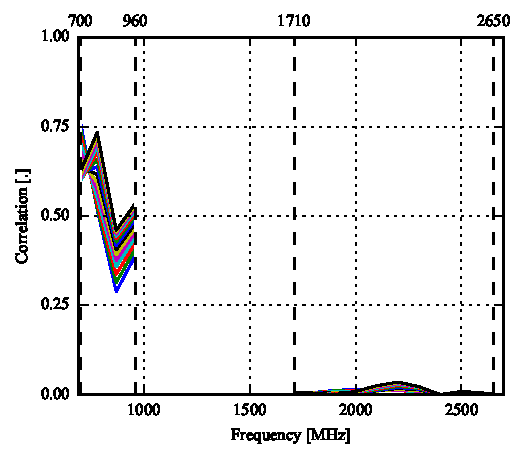
\includegraphics[width=0.78\linewidth]{img/henrik/mono/s11_corr} \\
    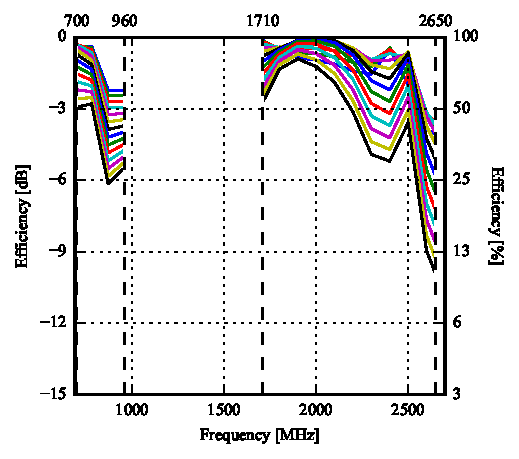
\includegraphics[width=0.82\linewidth]{img/henrik/mono/efficiency-ac1-csh1} 

  \end{minipage}\hfill       
  \begin{minipage}[t]{0.49\linewidth}
    \vspace{0 mm}

    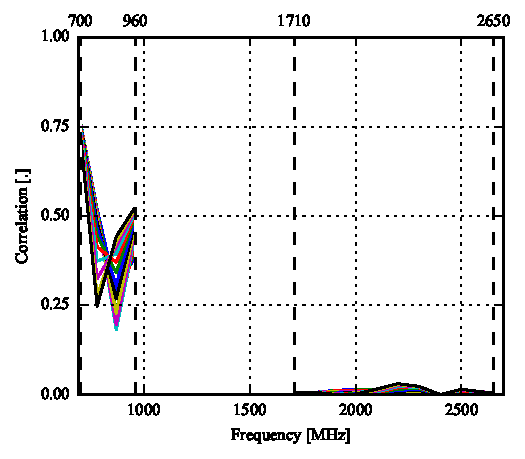
\includegraphics[width=0.78\linewidth]{img/henrik/mono/s22_corr} \\
    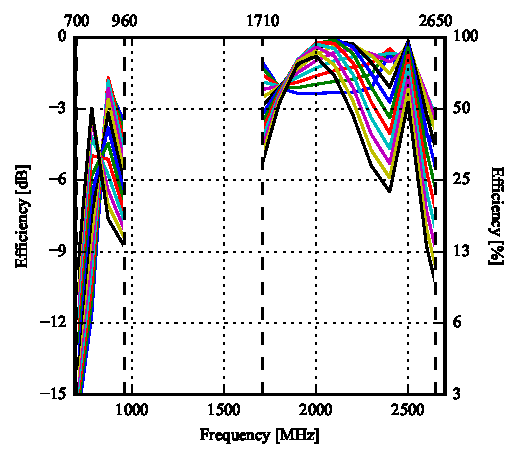
\includegraphics[width=0.82\linewidth]{img/henrik/mono/efficiency-ac2-csh2} 

  \end{minipage}    
\end{frame}



\begin{frame}
    \frametitle{Free-space simulations -- Triangle-feed (S-parameters)}
    \vspace*{-0.5cm}
  \begin{minipage}[t]{0.49\linewidth}
    \vspace{0mm}

    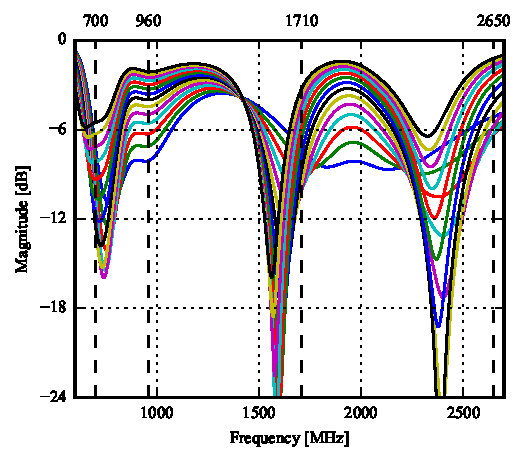
\includegraphics[width=0.78\linewidth]{img/henrik/triag/Csh1s11.pdf} \\
    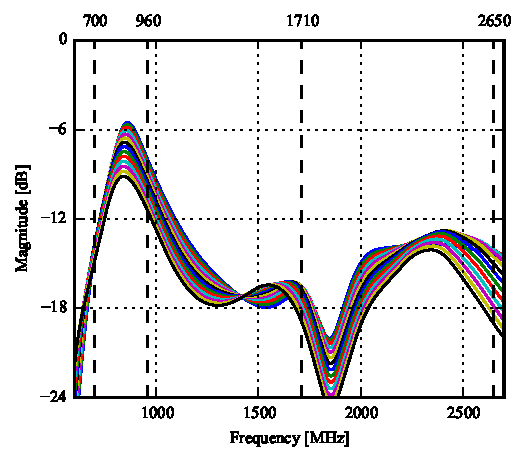
\includegraphics[width=0.78\linewidth]{img/henrik/triag/Csh1s21.pdf} 

  \end{minipage}\hfill       
  \begin{minipage}[t]{0.49\linewidth}
    \vspace{0 mm}

    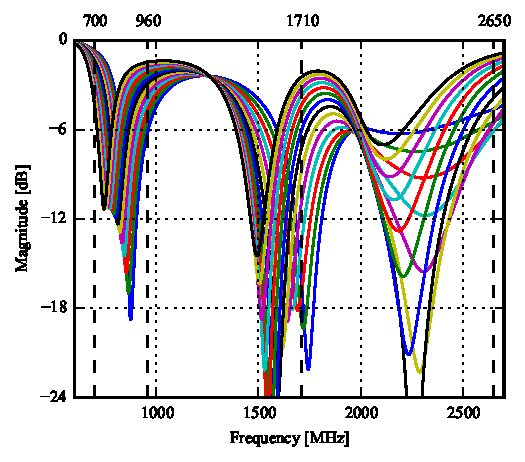
\includegraphics[width=0.78\linewidth]{img/henrik/triag/Csh2s22.pdf} \\
    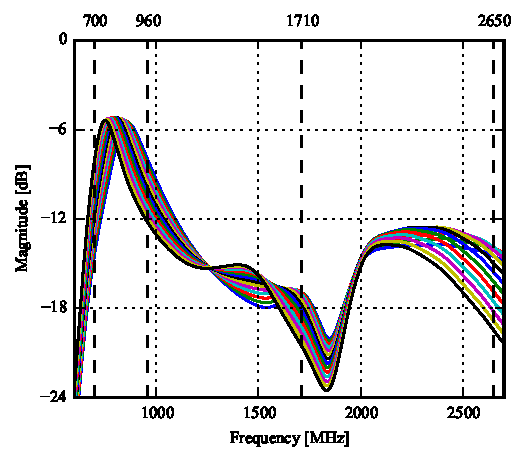
\includegraphics[width=0.78\linewidth]{img/henrik/triag/Csh2s21.pdf} 

  \end{minipage}    


\end{frame}

\begin{frame}
    \frametitle{Free-space simulations -- Triangle-feed (Efficiency and correlation)}
    \vspace*{-0.5cm}
  \begin{minipage}[t]{0.49\linewidth}
    \vspace{0mm}

    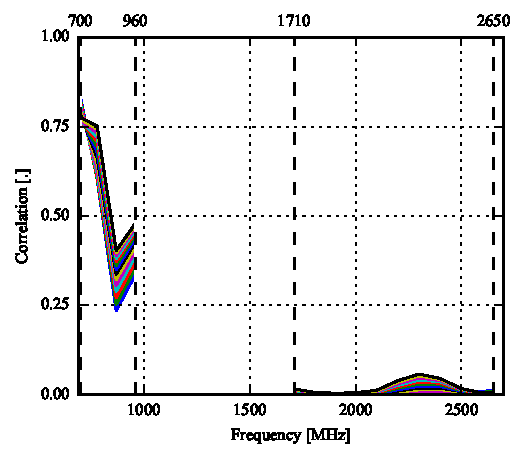
\includegraphics[width=0.78\linewidth]{img/henrik/triag/correlation_Csh1-sweep} \\
    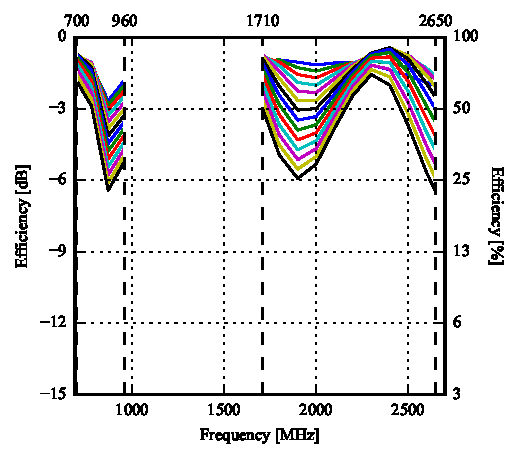
\includegraphics[width=0.78\linewidth]{img/henrik/triag/efficiency-ac1-csh1.pdf} \\



  \end{minipage}\hfill       
  \begin{minipage}[t]{0.49\linewidth}
    \vspace{0 mm}

    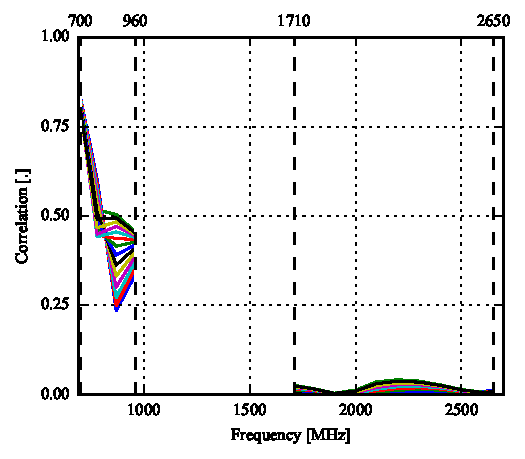
\includegraphics[width=0.78\linewidth]{img/henrik/triag/correlation_Csh2-sweep} \\
    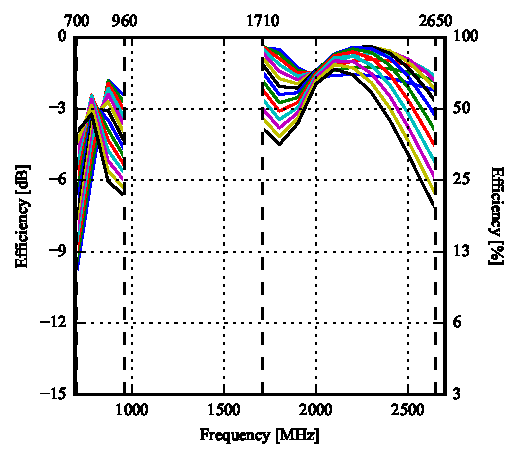
\includegraphics[width=0.78\linewidth]{img/henrik/triag/efficiency-ac2-csh2.pdf} 


  \end{minipage}    

\end{frame}


\begin{frame}
    \frametitle{Free-space simulations -- Dual-port (S-parameters)}

    \vspace*{-0.5cm}
  \begin{minipage}[t]{0.49\linewidth}
    \vspace{0mm}

    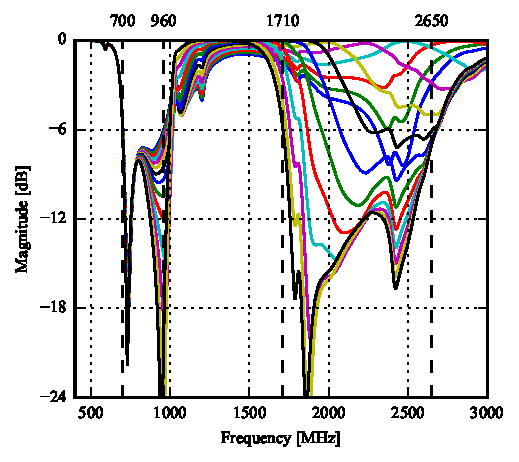
\includegraphics[width=0.78\linewidth]{img/henrik/dp/s11_top_sweep.pdf} \\
    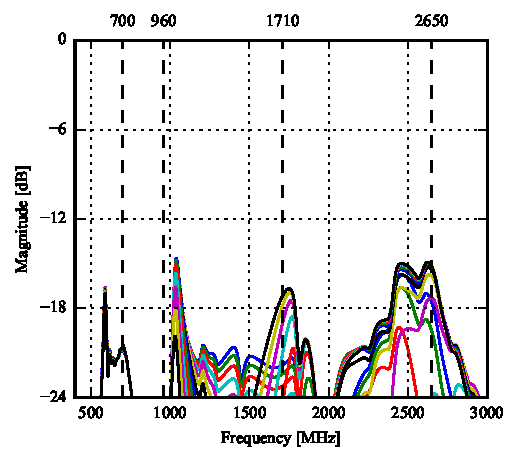
\includegraphics[width=0.78\linewidth]{img/henrik/dp/s12_top_sweep.pdf} 

  \end{minipage}\hfill       
  \begin{minipage}[t]{0.49\linewidth}
    \vspace{0 mm}

    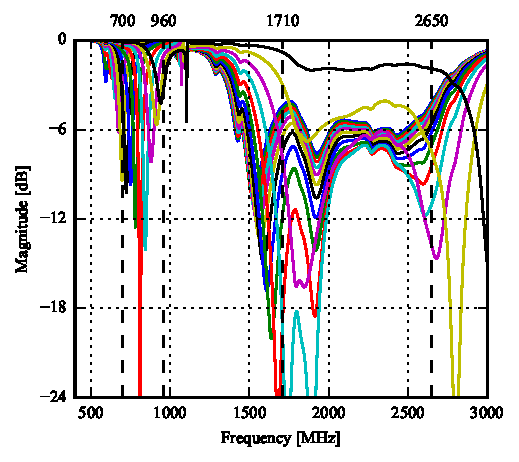
\includegraphics[width=0.78\linewidth]{img/henrik/dp/s22_side_sweep.pdf} \\
    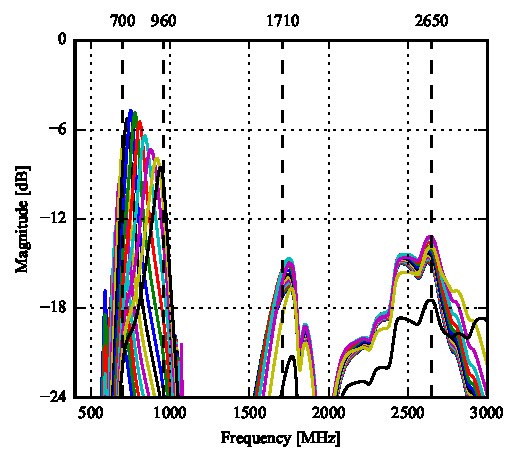
\includegraphics[width=0.78\linewidth]{img/henrik/dp/s21_side_sweep.pdf} 

  \end{minipage}    



\end{frame}

\begin{frame}
    \frametitle{Free-space simulations -- Dual-port (Efficiency and correlation)}
    \vspace*{-0.5cm}
  \begin{minipage}[t]{0.49\linewidth}
    \vspace{0mm}

    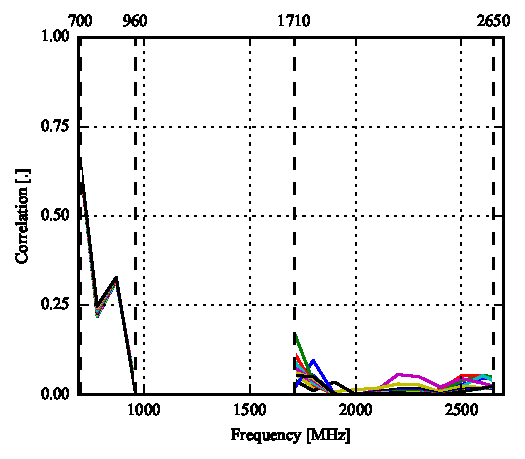
\includegraphics[width=0.78\linewidth]{img/henrik/dp/sweep_top_corr} \\
    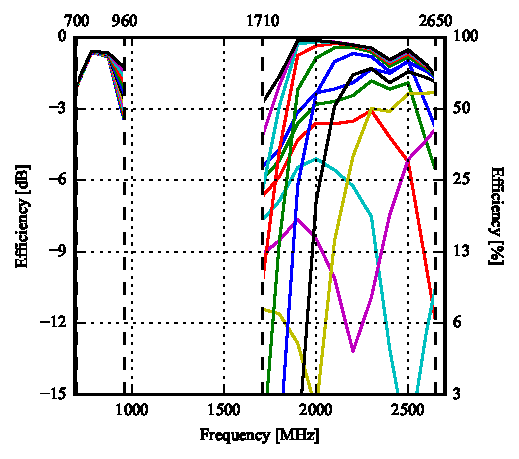
\includegraphics[width=0.78\linewidth]{img/henrik/dp/efficiency-ac2-top.pdf} 

  \end{minipage}\hfill       
  \begin{minipage}[t]{0.49\linewidth}
    \vspace{0 mm}

    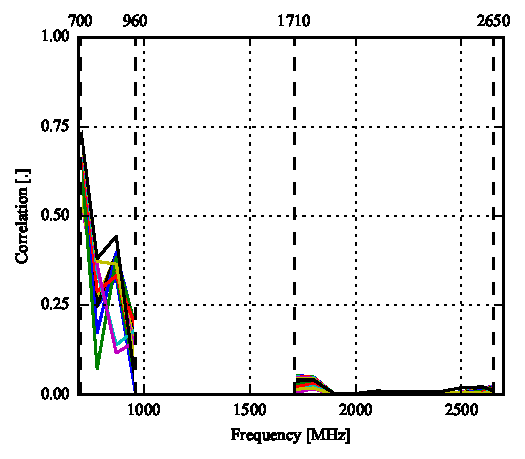
\includegraphics[width=0.78\linewidth]{img/henrik/dp/sweep_side_corr} \\
    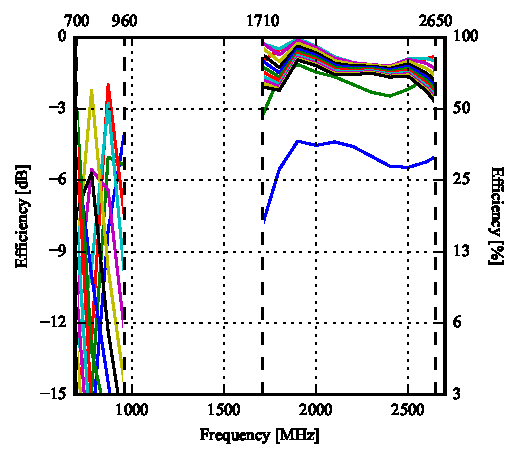
\includegraphics[width=0.78\linewidth]{img/henrik/dp/efficiency-ac3-side.pdf} 

  \end{minipage}    

\end{frame}










\section[User Effects]{User Effects (Søren)}
% Illustration of setup/positions on slide 1
% One slide for each:
    % All S11 on slide 2 
    % All S22 on slide 3
    % All S21 on slide 4
    % All efficiency on slide 5
    % All correlation on slide 6
    % All SAR on slide 7 (only one figure)
% For each slide, three figures/subplot (for each design)
    % Blue (freespace[0]), alpha 0.5 (min(freespace))
    % Green (data[0]), alpha 0.5 (min(data))
    % Red (play[0]), alpha 0.5 (min(play))
    % Cyan (talk[0]), alpha 0.5 (min(talk))

\def\legendfooter{\scriptsize{(1) Monopole (2) Triangle-feed (3) Dual-feed. \textcolor{bb}{Free-space}, \textcolor{gg}{Data}, \textcolor{rr}{Play}, \textcolor{cc}{Talk}. Frequency in MHz.}}
\def\emptyline{\textcolor{white}{Empty}}
\begin{frame}
    \frametitle{User Effects}
    \begin{columns}[onlytextwidth,T]
        \column{0.49\linewidth}
        Color codes: \vspace{0pt}
        \begin{tabular}{m{1in}m{3in}}
            \rule{0in}{0.3in} & \textcolor{bb}{Free space}\\
            \centering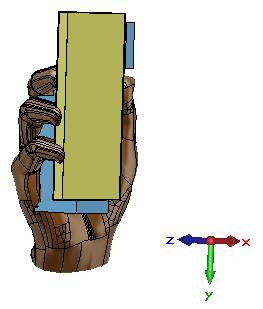
\includegraphics[height=0.6in, keepaspectratio]{img/soren/ue/usereff_onehand} & \textcolor{gg}{Data mode} \\
            \centering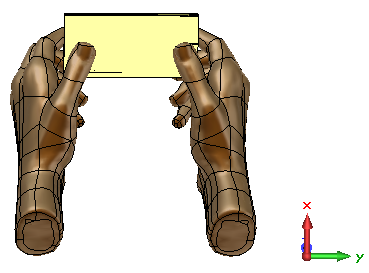
\includegraphics[height=0.6in, keepaspectratio]{img/soren/ue/usereff_twohand} & \textcolor{rr}{Play mode} \\
            \centering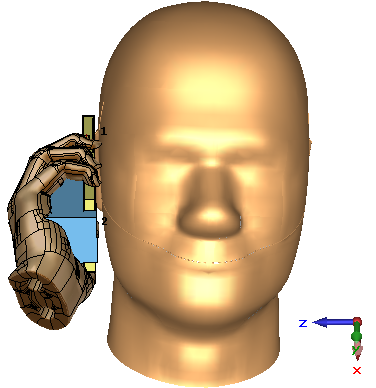
\includegraphics[height=0.6in, keepaspectratio]{img/soren/ue/usereff_headhand}& \textcolor{cc}{Talk mode}\\
            \centering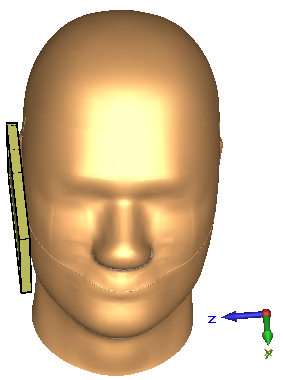
\includegraphics[height=0.6in, keepaspectratio]{img/soren/ue/usereff_sar}     & SAR
        \end{tabular}

        \column{0.49\linewidth}
        User effect simulations for the three designs.
        \begin{itemize}
            \item $S_{11}$, $S_{22}$, efficiency, correlation.
            \item All SAR $<\SI{2}{W/kg}$.
            \item Isolation not shown. See report.
        \end{itemize}

        Goal:
        \begin{itemize}
            \item Find the most stable design.
            \item Preserves bandwidth in use cases.
        \end{itemize}
    \end{columns}
\end{frame}

\begin{frame}
    \frametitle{User Effects -- S11, minimum over tunable range}
    % \emptyline
    Design 2 is generally is better matched.
    \begin{center}
        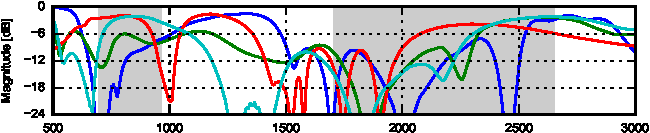
\includegraphics{img/soren/ue/design1lt/s11top.pdf}\\
        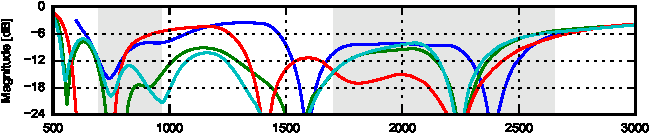
\includegraphics{img/soren/ue/design2sn/s11top.pdf}\\
        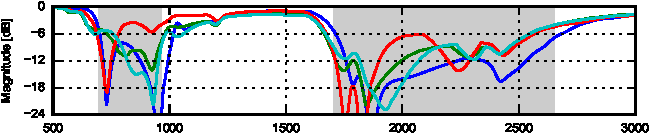
\includegraphics{img/soren/ue/design3hv/s11top.pdf}
    \end{center}
    \legendfooter
\end{frame}

\begin{frame}
    \frametitle{User Effects -- S22, minimum over tunable range}
    % \emptyline
    Detuning. Design 2 is better matched.
    \begin{center}
        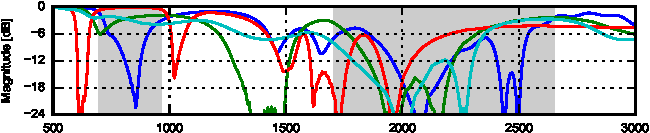
\includegraphics{img/soren/ue/design1lt/s22side.pdf}\\
        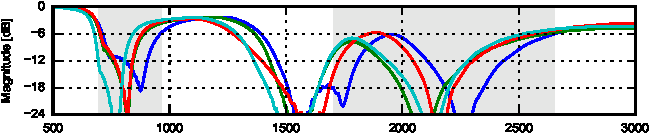
\includegraphics{img/soren/ue/design2sn/s22side.pdf}\\
        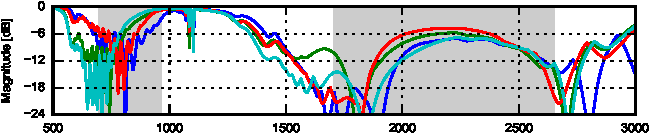
\includegraphics{img/soren/ue/design3hv/s22side.pdf}
    \end{center}
    \legendfooter
\end{frame}

\begin{frame}
    \frametitle{User Effects -- Total efficiency, minimum over tunable range (top)}
    % \emptyline
    Design 2 and 3 is better.
    \begin{center}
        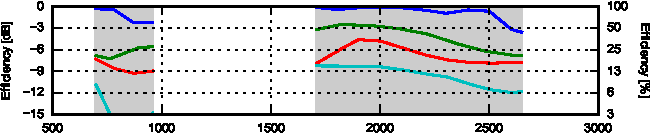
\includegraphics{img/soren/ue/design1lt/efftop.pdf}\\
        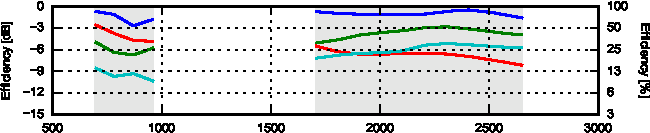
\includegraphics{img/soren/ue/design2sn/efftop.pdf}\\
        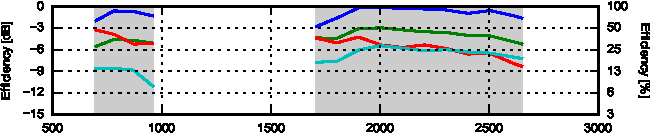
\includegraphics{img/soren/ue/design3hv/efftop.pdf}
    \end{center}
    \legendfooter
\end{frame}

\begin{frame}
    \frametitle{User Effects -- Total efficiency, minimum over tunable range (side)}
    % \emptyline
    Design 2 is better.
    \begin{center}
        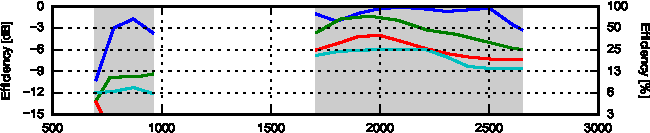
\includegraphics{img/soren/ue/design1lt/effside.pdf}\\
        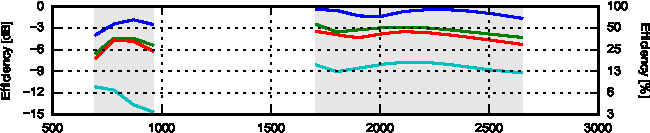
\includegraphics{img/soren/ue/design2sn/effside.pdf}\\
        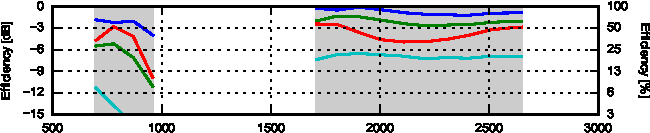
\includegraphics{img/soren/ue/design3hv/effside.pdf}
    \end{center}
    \legendfooter
\end{frame}

\begin{frame}
    \frametitle{User Effects -- Correlation, minimum over tunable range (tuning top)}
    Increase and decrease in correlation for different use cases.
    \emptyline
    \begin{center}
        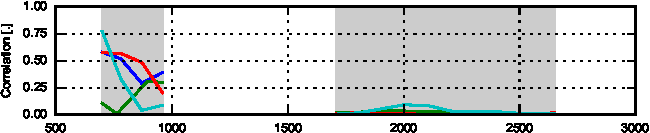
\includegraphics{img/soren/ue/design1lt/corrtop.pdf}\\
        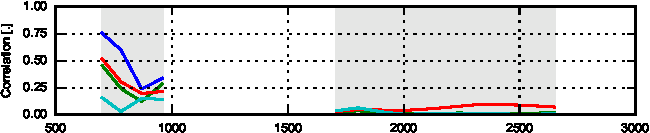
\includegraphics{img/soren/ue/design2sn/corrtop.pdf}\\
        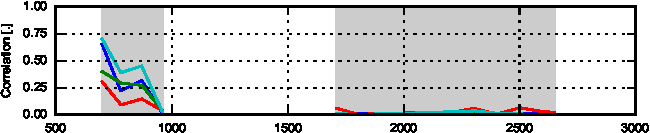
\includegraphics{img/soren/ue/design3hv/corrtop.pdf}
    \end{center}
    \legendfooter
\end{frame}

\begin{frame}
    \frametitle{User Effects -- Correlation, minimum over tunable range (tuning side)}
    Increase and decrease in correlation for different use cases.
    \emptyline
    \begin{center}
        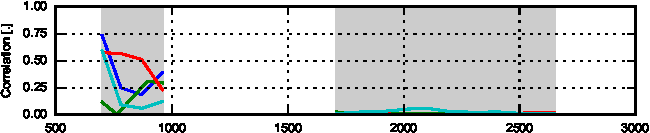
\includegraphics{img/soren/ue/design1lt/corrside.pdf}\\
        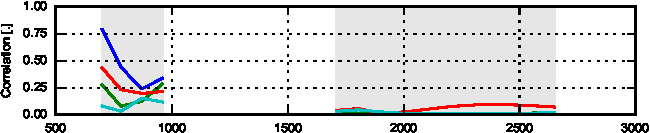
\includegraphics{img/soren/ue/design2sn/corrside.pdf}\\
        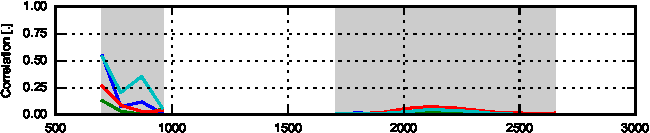
\includegraphics{img/soren/ue/design3hv/corrside.pdf}
    \end{center}
    \legendfooter
\end{frame}

\begin{frame}
    \frametitle{User Effects -- Preliminary Conclusion}
    \begin{tabular}{m{0.4in}m{4in}}
        \rule{0pt}{0.9in}\includegraphics[height=0.75in]{img/soren/1st.pdf} & 
            Design 2 -- triangle-feed
            \begin{itemize}
                \item Better efficiency and impedance bandwidth.
                \item High free-space correlation in low band. 
            \end{itemize}
            \\
        \rule{0pt}{0.9in}\includegraphics[height=0.75in]{img/soren/2nd.pdf} & 
            Design 3 -- dual-feed
            \begin{itemize}
                \item More fluctuating than design 2.
                \item Still good bandwidth/efficiency.
            \end{itemize}
            \\
        \rule{0pt}{0.9in}\includegraphics[height=0.75in]{img/soren/3rd.pdf} & 
            Design 1 -- monopole
            \begin{itemize}
                \item Very sensitive to user effects.
                \item Low efficiency and impedance bandwidth.
            \end{itemize}
    \end{tabular}
\end{frame}

\section[Prototypes]{Prototypes (Søren)}
\begin{frame}
    \frametitle{Prototypes}
    \begin{columns}[onlytextwidth,T]
        \vspace{0em}
        \column{0.49\linewidth}
        \begin{tabular}{m{0.3in}m{1.4in}}
             (1) & \includegraphics[width=1.4in]{img/soren/proto/design1}\\
             (2) & \includegraphics[width=1.4in]{img/soren/proto/design2}\\
             (3) & \includegraphics[width=1.4in]{img/soren/proto/design3}
        \end{tabular}

        \column{0.49\linewidth}
        Prototypes of the three designs.
        \begin{itemize}
            \item $S_{11}$, $S_{22}$, efficiency.
            \item Isolation not shown. See report.
        \end{itemize}

        Goal:
        \begin{itemize}
            \item Find most realizable design.
            \item Verify simulation results -- useful design in real life?
        \end{itemize}
    \end{columns}
\end{frame}

\def\legendfooter{\scriptsize{Upper: Top antenna. Lower: Side antenna. Frequency in MHz.}}
\begin{frame}
    \frametitle{Prototype 1 -- Monopole}
    High band moves a lot during tuning.
    % \emptyline
    \begin{center}
        \includegraphics{img/soren/proto/design1lt/s11.pdf}
        \includegraphics{img/soren/proto/design1lt/efftop.pdf}\\
        \includegraphics{img/soren/proto/design1lt/s22.pdf}
        \includegraphics{img/soren/proto/design1lt/effside.pdf}
    \end{center}
    \legendfooter
\end{frame}

\begin{frame}
    \frametitle{Prototype 2 -- Triangle-feed}
    \textcolor{gg}{High bandwidth!} High band stable over multiple capacitances.
    % \emptyline
    \begin{center}
        \includegraphics{img/soren/proto/design2sn/s11.pdf}
        \includegraphics{img/soren/proto/design2sn/efftop.pdf}\\
        \includegraphics{img/soren/proto/design2sn/s22.pdf}
        \includegraphics{img/soren/proto/design2sn/effside.pdf}
    \end{center}
    \legendfooter
\end{frame}

\begin{frame}
    \frametitle{Prototype 3 -- Dual-feed}
    OK efficiency. Side antenna -- good but not tunable.
    % \emptyline
    \begin{center}
        \includegraphics{img/soren/proto/design3hv/s11.pdf}
        \includegraphics{img/soren/proto/design3hv/efftop.pdf}\\
        \includegraphics{img/soren/proto/design3hv/s22.pdf}
        \includegraphics{img/soren/proto/design3hv/effside.pdf}
    \end{center}
    \legendfooter
\end{frame}

\begin{frame}
    \frametitle{Prototypes -- Preliminary Conclusion}
    \begin{tabular}{m{0.4in}m{4in}}
        \rule{0pt}{0.9in}\includegraphics[height=0.75in]{img/soren/1st.pdf} & 
            Design 2 -- triangle-feed.
            \begin{itemize}
                \item Covers all bands at $C_{\text{low}}$.
                \item Preserves higher efficiency when tuned.
                \item \textit{Moved to tuner PCB}.
            \end{itemize}
            \\
        \rule{0pt}{0.9in}\includegraphics[height=0.75in]{img/soren/2nd.pdf} & 
            Design 3 -- dual-feed
            \begin{itemize}
                \item Top antenna good in most bands.
                \item Side antenna not tunable but good.
            \end{itemize}
            \\
        \rule{0pt}{0.9in}\includegraphics[height=0.75in]{img/soren/3rd.pdf} & 
            Design 1 -- monopole
            \begin{itemize}
                \item Covers low bands OK.
                \item Low efficiency when tuned.
            \end{itemize}
    \end{tabular}
\end{frame}

\section{Tuner PCB}
\begin{frame}
  \frametitle{Outline}
      \begin{itemize}
      \item Ground Clearance simulation.
      \item Tuner PCB with MEMS tuner.
        \begin{itemize}
        \item Triangle-Feed antenna.
        \item Modified monopole antenna.
        \end{itemize}
      \item Conclusion
      \end{itemize}
\end{frame}

\begin{frame}[fragile]
  \frametitle{Ground Clearance}
  \begin{columns}[onlytextwidth,t]
    \column{0.49\linewidth}
      \begin{itemize}
      \item Minimized and simplified monopole design.
      \item \SI{10}{mm} to \SI{5}{mm} ground clearance simulation
      \end{itemize}
    \column{0.49\linewidth}
    \begin{center}
      \includegraphics[scale=0.7]{img/Lasse/3d_drawing_mini.pdf}
    \end{center}
    Technical Drawing
  \end{columns}
\end{frame}

\begin{frame}
  \frametitle{Ground Clearance}
    \begin{center}
      \includegraphics[scale=0.7]{img/Lasse/s11_5mm.pdf}
\includegraphics[scale=0.7]{img/Lasse/eff_5mm.pdf}
    \end{center}
      \begin{itemize}
      \item Significant bandwidth and efficiency drop from \SI{5}{mm} to \SI{4}{mm}.
      \end{itemize}
\end{frame}

\begin{frame}[fragile]
    \frametitle{Tuner PCB}
    \begin{columns}[onlytextwidth,t]
        \column{0.49\linewidth}
          \begin{itemize}
          \item PCB with MEMS tuner.
          \end{itemize}
        \column{0.49\linewidth}
        \begin{center}
            \includegraphics[scale=0.33]{img/Lasse/samanthas_board.pdf}
        \end{center}
        Tuner PCB
    \end{columns}
\end{frame}

\begin{frame}
  \frametitle{Tuner PCB Results}
  \begin{itemize}
  \item Problems with detuning in the high frequencies.
  \end{itemize}
  \begin{center}
    \includegraphics[scale=0.33]{img/Lasse/tuner_pcb/001_s11top.pdf}
    \includegraphics[scale=0.33]{img/Lasse/tuner_pcb/001_s11side.pdf} \\
    \includegraphics[scale=0.33]{img/Lasse/tuner_pcb/001.pdf}
    \includegraphics[scale=0.33]{img/Lasse/tuner_pcb/.pdf}
  \end{center}
\end{frame}

\begin{frame}[fragile]
    \frametitle{Tuner PCB -- Modified Design}
    \begin{columns}[onlytextwidth,t]
        \column{0.49\linewidth}
          \begin{itemize}
          \item Adding of a higher resonant to counteract the detuning.
          \item Two arms added in the available space. 
          \item Ground clearance \SI{2.5}{mm}.
          \end{itemize}
        \column{0.49\linewidth}
        \begin{center}
            \includegraphics[scale=0.33, angle =90]{img/Lasse/lassedouble.pdf}
            \includegraphics[scale=0.53]{img/Lasse/3d_drawing_modi.pdf}
        \end{center}
        Tuner PCB with the modified monopole.
    \end{columns}
\end{frame}

\begin{frame}
  \frametitle{Tuner PCB}
    \begin{block}{Modified Monopole Results.}
      \begin{itemize}
      \item Results of the added resonant.
      \item Simulation results.
      \item Measurement results.
      \item Shunt capacitor on transmission lines.
      \end{itemize}
    \end{block}
\end{frame}

\begin{frame}
  \frametitle{Conclusion}
      \begin{itemize}
      \item Three preliminary designs.
      \item Two designs on the tuner PCB.
      \item Modified \SI{2.5}{mm} ground clearance design.
    \item Promising prototype results comparable with state-of-the-art designs.
    \item Problems with the resonance in the higher frequencies.
    \item MIMO support in the high band -- high correlation in the low band.
      \end{itemize}
\end{frame}


\end{document}
